\section{Namespace: Logik laget}

\begin{figure}[H]
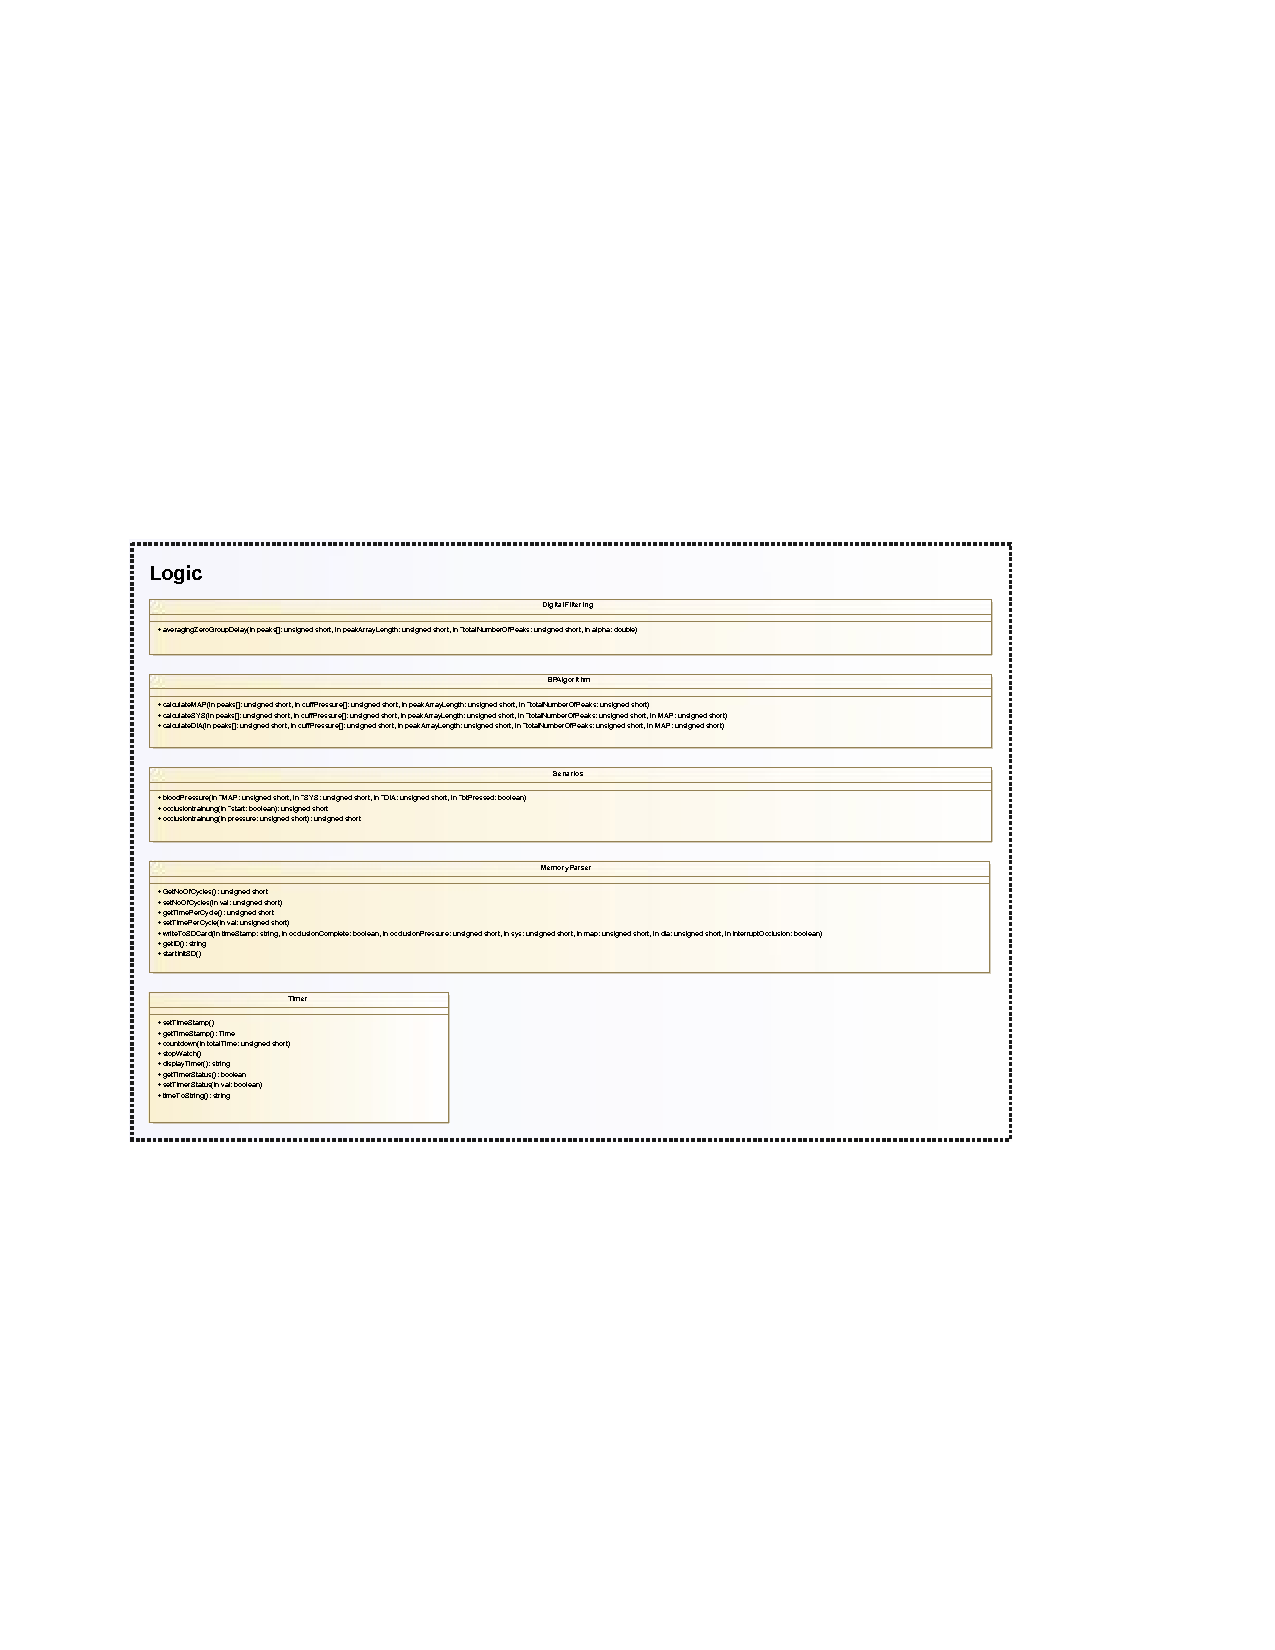
\includegraphics[trim = 0 170 0 0, clip = true, width=\textwidth]{klassediagram_Logic-crop.pdf}
\caption{Klasse diagram over namespacet Logic}\label{fig:classDiagramLogic}
\end{figure}

\subsection{Klasse: BPalgorithm}

\subsubsection{Metode: calculateMap()}
\textbf{Parameter: } \textit{unsigned short peaks[], unsigned short cuffPressure[], unsigned short peakArrayLength, unsigned short *totalNumberOfPeaks}
\\ \textbf{Returtype: } \textit{unsigned short}
\\ \textbf{Beskrivelse: } Denne metode beregner MAP ud fra digitalt filtreret peakdata i peaks[] og cuffPressure[]. MAP findes som trykket i manchetten ved den højeste peak amplitude (se figur \ref{fig:bpMeasurement})

\newpage
\begin{figure}[H]
	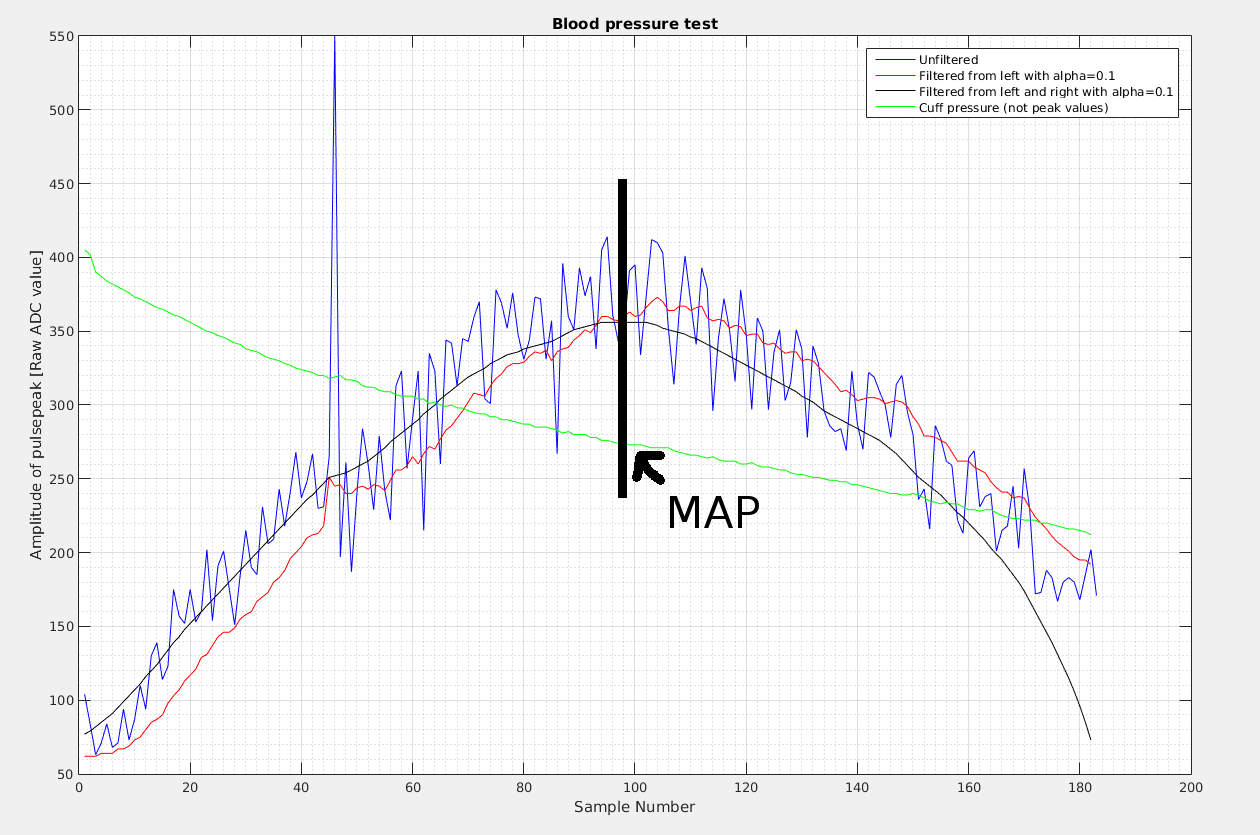
\includegraphics[width=\textwidth]{billeder/4_11_2016.png}
	\caption{Graf med data fra en blodtryksmåling}\label{fig:bpMeasurement}
\end{figure}
Her ses at det rå signal er støjfyldt. Grøn er manchet trykket, blå er de rå peak amplituder, rød er filtreret en gang fra venstre mod højre, sort	er filtreret fra begge sider.

\subsubsection{Metode: calculateSYS()}
\textbf{Parameter: } \textit{unsigned short peaks[], unsigned short cuffPressure[],unsigned short peakArrayLength, unsigned short *totalNumberOfPeaks, unsigned short MAP}
\\ \textbf{Returtype: } \textit{unsigned short}
\\ \textbf{Beskrivelse: } Denne metode beregner SYS ud fra MAP og digitalt filtreret peakdata i peaks[] og cuffPressure[]. SYS findes som trykket i manchetten ved peak amplituder på 31\% af MAP.

\subsubsection{Metode: calculateDIA()}
\textbf{Parameter: } \textit{unsigned short peaks[], unsigned short cuffPressure[],unsigned short peakArrayLength, unsigned short *totalNumberOfPeaks, unsigned short MAP}
\\ \textbf{Returtype: } \textit{unsigned short}
\\ \textbf{Beskrivelse: } Denne metode beregner DIA ud fra MAP og digitalt filtreret peakdata i peaks[] og cuffPressure[]. DIA findes som trykket i manchetten ved peak amplituder på 52 \% af MAP. 

\subsection{Klasse: DigitalFiltering}

\subsubsection{Metode: averagingZeroGroupDelay()}
\textbf{Parameter: } \textit{nsigned short peaks[],unsigned short peakArrayLength, unsigned short *totalNumberOfPeaks, double alpha}
\\ \textbf{Returtype: } \textit{void}
\\ \textbf{Beskrivelse: } Denne metode anvender eksponentiel midligsfilter teknik (Se afsnit \ref{title:digitalFilter}) uden group delay til at midle over parameteren peaks.
\begin{lstlisting}
	peaks[0] = startValue;
	peaks[totalNOPeaks] = startValue;
	for(i = 1;i<totalNOPeaks; i++)
	{
	peaks[i] = alpha*peaks[i]+(1-alpha)*peaks[i-1];
	}
	
	for(i = totalNOPeaks-1;i>0; i--)
	{
	peaks[i] = alpha*peaks[i]+(1-alpha)*peaks[i+1];
	}
\end{lstlisting}

\subsection{Klasse: Scenarios}

\subsubsection{Metode: bloodPressure()}
\textbf{Parameter: } \textit{unsigned short *MAP, unsigned short *SYS, unsigned short *DIA, BPAlgorithm bpa, Data::PressureControl pc, Data::PressureSampling ps, Logic::DigitalFiltering df, Utilities util}
\\ \textbf{Returtype: } \textit{void}
\\ \textbf{Beskrivelse: } Denne metode indeholder opskriften til en blodtryksmåling. Det vil sige at kaldes metoden, udføres en blodtryksmåling og alle andre klasser og metoder, som skal bruges til dette eksekveres inde i denne metode. Pointerne til de tre variabler får værdierne MAP, SYS og DIA fra blodtryksmålingen.

\subsection{Klasse: Timer}
Klassen timer gør brug af en hardware Real Time Clock(RTC) med IC’en \textit{DS1302}. For at kommunikere med denne RTC, så gør klassen brug af et biblioteket \textit{DS1302}. Derfor oprettes et objekt af klassen \textit{DS1302.h} ved navn timestamp. Et Time objektet indeholder hhv: år, måned, dag, time, minut, sekund og ugedag. 

\subsubsection{Metode: setTimeStamp()}
\textbf{Parameter: } 
\\ \textbf{Returtype: } \textit{void}
\\ \textbf{Beskrivelse: } Denne metode aflæser den nuværende værdi af timeren og sætter en variable til denne værdi. 

\subsubsection{Metode: getTimeStamp()}
\textbf{Parameter: } 
\\ \textbf{Returtype: } \textit{Time}
\\ \textbf{Beskrivelse: } Returnerer et Time objekt med værdien af timestamp. 

\subsubsection{Metode: countdown()}
\textbf{Parameter: } \textit{unsigned short totalTime}
\\ \textbf{Returtype: } \textit{void}
\\ \textbf{Beskrivelse: } Denne metode modtager parameteren \textit{totalTime}, som indeholder det ønskede antal sekunder nedtællingen skal vare. Variablen \textit{elapsedTime} indeholder den nuværende tid og timestamp indeholder et tidsstempel der bliver sat når timeren skal starte. Hver gang metoden køres trækkes den nuværende tid i hhv timer, minutter og sekunder fra hinanden. Dernæst omregnes de forskellige difference til samlede antal sekunder, hvorefter det tal omregnes til sekunder og minutter. For at få antal sekunder tages differencen mellem \textit{totalTime} og \textit{elapsedTotalSeconds} udregner modulus 60 til dette tal(Se formel \ref{eq:totalSeconds})
\begin{equation} \label{eq:totalSeconds}
seconds = (totalTime - elapsedTotalSeconds) \bmod 60
\end{equation}

Dette samme gøres for minutter blot hvor \textit{seconds} også trækkes fra. Se kode nedenfor. 
\begin{lstlisting}
	timerHasEnded = false;
	Time elapsedTime = rtc.time();
	String elapsedTimeString;
	unsigned short hoursToSec = (elapsedTime.hr-timestamp.hr) * 24	* 60;
	unsigned short minutesToSec = (elapsedTime.min- timestamp.min)	* 60;
	unsigned short elapsedTotalSeconds = hoursToSec + minutesToSec	+ (elapsedTime.sec - timestamp.sec);
	seconds = (totalTime - elapsedTotalSeconds) % 60;
	minutes = (totalTime - elapsedTotalSeconds - seconds)/60;
	
	if(minutes == 0 && seconds == 0)
	timerHasEnded = true;
\end{lstlisting}
Når det er regnet ud hvor mange minutter og sekunder der er tilbage i nedtællingen, gemmes de lokale variable minutes og seconds. 

\subsubsection{Metode: stopWatch()}
\textbf{Parameter: } 
\\ \textbf{Returtype: } \textit{void}
\\ \textbf{Beskrivelse: } Metode til at styre simulere og styre et stopur under okklusionstræning, den forløbne tid udregnes på samme måde \textit{countdown()}, blot hvor det er tidsstemplet der trækkes fra den nuværende tid. Denne metode gemmer også minutter og sekunder i to lokale variabler, når udregning er den forløbne tid er færdig. 

\subsubsection{Metode: displayTimer()}
\textbf{Parameter: }
\\ \textbf{Returtype: } \textit{ String}
\\ \textbf{Beskrivelse: } Denne metode bruges til at konvertere tiden fra enten stopuret eller nedtællingen til formatet mm:ss. Desuden konverteres tiden til en string. 
\begin{lstlisting}
	String minString = String(minutes, DEC);
	String secString = String(seconds, DEC);
	String timeString;
	
	if(0 <=minutes && minutes < 10)
	minString = String("0" + minString);
	else
	minString = String(minutes, DEC);
	
	if(0 <=seconds && seconds < 10)
	secString = String("0" + secString);
	else
	secString = String(seconds, DEC);
	return timeString = String(minString + ":" + secString);
\end{lstlisting}
For at sikre at tiden vises på formatet mm:ss, tjekker metoden for om \textit{seconds} eller \textit{minutes} er større eller lig med 0 og mindre end 10. Hvis det er tilfældet tilføjes et nul foran værdien 

\subsubsection{Metode: getTimerStatus()}
\textbf{Parameter: } 
\\ \textbf{Returtype: } \textit{bool}
\\ \textbf{Beskrivelse: } Metode til at returnere værdien af statussen for timeren, hvis værdien er sand er timeren slut og omvendt hvis værdien er falsk kan timeren stadig være igangværende. 

\subsubsection{Metode: setTimerStatus()}
\textbf{Parameter: } \textit{bool val}
\\ \textbf{Returtype: } \textit{void}
\\ \textbf{Beskrivelse: } Denne metode bruges til at sætte værdien af statussen for timeren, den sættes til true for at stoppe timeren. Derfor modtager en metode en parameter af typen bool. 

\subsubsection{Metode: timeToString()}
\textbf{Parameter: } 
\\ \textbf{Returtype: } \textit{String}
\\ \textbf{Beskrivelse: } For at kunne gemme tidsstempler på SD kortet, er denne metode lavet til at konvertere et tidsstempel til en string på formatet: \textit{tt:mm:ss DD-MM-YY}. Ligesom metoden \textit{displayTimer()} håndterer denne metode hvis enten timer, minutter eller sekunder er mindre end 10 og sætter et nul foran. Metoden returnere en samlede string med et tidsstempel 

\subsection{Klasse: MemoryParser}
Denne klasse er lavet for at overholde 3-lags modellen. Da informations læsning fra fx EEPROM og SD kort skal foregå i data laget, skal der en række metoder til at sende information igennem logik laget og videre til GUI laget. Derfor indeholder denne klasse som udgangspunkt kun get og set metoder. 

\subsubsection{Metode: getNoOfCycles()}
\textbf{Parameter: } 
\\ \textbf{Returtype: } \textit{unsigned short}
\\ \textbf{Beskrivelse: } Denne metode returnere værdien fra data laget via metoden \textit{“intMem.readFromEEPROM()”}.

\subsubsection{Metode: setNoOfCycles()}
\textbf{Parameter: } \textit{unsigned short val}
\\ \textbf{Returtype: } \textit{void}
\\ \textbf{Beskrivelse: } Metode der skriver til data laget via metoden: \textit{intMem.writeToEEPROM(200, val)}. Parameteren \textit{val} videres til med denne metode. 

\subsubsection{Metode: getTimePerCycle()}
\textbf{Parameter: } 
\\ \textbf{Returtype: } \textit{unsigned short}
\\ \textbf{Beskrivelse: } Da værdien af timePerCycle indeholder hvor mange sekunder én konditioneringscyklus skal vare, er denne værdi ofte større end 255. Denne værdi skal læses fra EEPROM og en plads kan indeholde værdier på maks 255. Derfor sørger metoden for at hente værdien fra den anden plads, hvis den er større end maks værdien. 
\begin{lstlisting}
	unsigned short val = intMem.readFromEEPROM(205);
	unsigned overloadVal = 0;
	if(val == 255)
	return overloadVal = val + intMem.readFromEEPROM(206);
	else
	return val;
\end{lstlisting}


\subsubsection{Metode: setTimePerCycle()}
\textbf{Parameter: } \textit{unsigned short val}
\\ \textbf{Returtype: } \textit{void}
\\ \textbf{Beskrivelse: } Beskrivelse: Når denne metode køres skrives tiden pr. cyklus til EEPROM, som forklaring i metoden \textit{getTimePerCycle()}, skal den metode håndtere overload. 
\begin{lstlisting}
	if(val > 255){
	unsigned short rest = val % 255;
	unsigned short valtoFit = val - rest;
	intMem.writeToEEPROM(205, valtoFit);
	intMem.writeToEEPROM(206, rest);
	}
	else
	intMem.writeToEEPROM(205, val);
\end{lstlisting}
Det er forinden bestemt at adresserne 205 og 206 bruges til at gemme \textit{TimePerCycle}. Metoden får en parameter som indeholder antallet af sekunder en cyklus skal vare, og for sørge for værdien skrives korrekt til EEPROM udregnes modulus 255 af antallet af sekunder og den rest gemmes på adressen 206. 

String timeStamp, boolean occlusionComplete, unsigned short occlusionPressure, unsigned short sys, unsigned short map, unsigned short dia, boolean interruptOcclusion

\subsubsection{Metode: writeToSDCard()}
\textbf{Parameter: } \textit{String timeStamp, boolean occlusionComplete, unsigned short occlusionPressure, unsigned short sys, unsigned short map, unsigned short dia, boolean interruptOcclusion}
\\ \textbf{Returtype: } \textit{void}
\\ \textbf{Beskrivelse: }  Denne metode indeholder syv parametre af typerne \textit{String}, \textit{boolean} og \textit{unsigned short}. Metoden konverterer og samler alle parametrene til en string og ved denne sendes videre til datalaget.